\documentclass[10pt,A4]{article} % Use the custom resume.cls style

\usepackage{verbatim} % usefull to coment out blocs
\usepackage{graphics}
\usepackage{wrapfig}
\usepackage{mycv}

% Define title and author
\title{Curriculum Vitae}
\author{Ant\^onio Horta Ribeiro}
\date{}


\begin{document}

\maketitle
\small



\section{Personal Information}

\begin{itemize}
\item {\bf Birthdate and place:} 1992-10-21, Brazil.
\item {\bf Emails and phone number:} antonio.horta.ribeiro@it.uu.se,  + 46 70 254 42 85
\item {\bf Visiting address:}  Ångströmslaboratoriet, Hus 10, Room 103179
\item {\bf Postal address:} Box 337, 751 05, Uppsala, Sweden.
\item {\bf Website:} antonior92.github.io.
\end{itemize}

\section{Current Employment}

\begin{itemize}
\item \shortcventry{ Assistant Professor}
    { June 2024 -  Now }
    { Uppsala University,  }{}{}
\end{itemize}



\section{Degrees}


\begin{itemize}

    \item \shortcventry{ Ph.D., Electrical Engineering }
    { Mar. 2020 }
    { Universidade Federal de Minas Gerais (UFMG), Brazil }{}

    \item \shortcventry{ M.Sc., Electrical Engineering }
    { Jul. 2017 }
    { Universidade Federal de Minas Gerais (UFMG), Brazil }{}

    \item \shortcventry{ B.S.E., Electrical Engineering }
    { Jul. 2017 }
    { Universidade Federal de Minas Gerais (UFMG), Brazil }{}

\end{itemize}

\section{Postdoctoral training} % Section title

\begin{itemize}

    \item \shortcventry{ Postdoctoral Associate }
    { Fev. 2022 -   May 2024  }
    { KTH Royal Institute of Technology,   }{}{} Hosted by Danica Kragic.

    \item \shortcventry{ Postdoctoral Fellow }
    { Fev. 2021 -   Jan. 2023  }
    { Uppsala University, Sweden  }{}{} Hosted by Thomas Schön

    \item \shortcventry{ Visiting Researcher }
    { Mar 2023 -   June 2023  }
    { INRIA, Sweden  }{}{} Hosted by Francis Bach.

    \item \shortcventry{ Postdoctoral Associate }
    { Mar. 2020 -   Fev. 2021  }
    { UFMG, Brazil  }{}{} Funded by CAPES PRiNT

\end{itemize}
  

\section{Awards}

\begin{itemize}

    \item \shortcventry{ Benzelius award }
    { 2022 }
    { Royal Society of Sciences in Uppsala }
    { Sweden }
    { I was awarded the Benzelius Award (Benzeliusbelöningarna) due to my 'contributions to fundamental method development in machine learning and control technology, as well as its use to solve important problems in cardiology'. The prize is awarded yearly by the Royal Society of Sciences in Uppsala (Kungliga Vetenskaps-Societeten i Uppsala): the oldest of the royal academies in Sweden, founded in 1710. Named after Erik Benzelius, the prize is awarded to young researchers and comes with the amount of 25000 kronors. }

    \item \shortcventry{ Best Ph.D. Thesis in Engineering and Physical Sciences }
    { 2021 }
    { Universidade Federal de Minas Gerais }
    { Belo Horizonte, Brazil }
    { My Ph.D. thesis was awarded the best Ph.D. thesis defended in 2020 in engineering and physical sciences at the Universidade Federal de Minas Gerais (UFMG), Brazil. In portuguese: Grande Premio de Teses na área de ciências exatas e da terra e engenharias. }

    \item \shortcventry{ Best Ph.D. Thesis in Electrical Engineering }
    { 2021 }
    { Universidade Federal de Minas Gerais }
    { Belo Horizonte, Brazil }
    { My thesis was awarded the best Ph.D. thesis defended in 2020 in the Department of Electrical Engineering at the Universidade Federal de Minas Gerais (UFMG), Brazil. The thesis was then forwarded to compete with the thesis from all other Engineering and Physical Sciences departments at the university (where it was also awarded the best thesis, see the award above). }

    \item \shortcventry{ Young Author Award (Honorable Mention) }
    { 2021 }
    { 19th IFAC Symposium on System Identification }
    { Online }
    { I have been one of the three finalists of the Young Author Award with the paper `Beyond Occam’s Razor in System Identification:  Double-Descent when Modeling Dynamics'. }

    \item \shortcventry{ Best Poster Award }
    { 2019 }
    { SciLifeLab Science Summit }
    { Uppsala, Sweden }
    { I have been awarded the best poster award for the work `Automatic Diagnosis of Short-Duration 12-Lead ECG using a Deep Convolutional Network'. }

    \item \shortcventry{ Travel Award }
    { 2018 }
    { Machine Learning for Health (ML4H) Workshop at NeurIPS }
    { Montreal, Canada }
    { I have been awarded the travel award for the work `Automatic Diagnosis of Short-Duration 12-Lead ECG using a Deep Convolutional Network' and had my expenses covered by the award. }

\end{itemize}
  

\section{Grants}
\subsection{Aquired external funding}

\begin{itemize}
\item \shortcventry{AI-ECG }{2022-2024}{CNPq (Brazil)  }{}{} {\small Co-applicant - 1 Million BRL ($\approx$ 200\,000 EUR)}

    \item \shortcventry{ CAPES-PRINT }
    { 2020-2021 }
    { CAPES (Brazil) }
    { Brazil }
    { I have been granted a scholarship from the Brasilian Agency CAPES for internacionalization. } {\small Main applicant-  60 Thousand BRL ($\approx$ 10\,000 EUR) }
  \end{itemize}

\subsection{Mobility grants}
\begin{itemize}
    \item \shortcventry{ UGhent mobility grant }
    { 2023 }
    { Ghent University - 10\,000 EUR }
    { Sweden }
    { Dirk Deschrijver and I were awarded a grant to estabilish international research collaboration. The budget will cover the travel expenses of PhD students to visit me at Uppsala Univeristy and work on automated ECG analysis. }
    \item \shortcventry{ SFVE-A mobility grant }
    { 2023 }
    { French Institute of Sweden - 1\,500 EUR }
    { Sweden }
    { I have been granted the Svensk Fransk Vetenskap–Anslag (SFVE-A) grant. }
   \item  \shortcventry{ ELISE mobility grant }
    { 2023 }
    { European Network of AI Excellence Centres - 2\,500 EUR}
    { Europe }
    { I have been granted for a research visit to Francis Bach group at ENS/INRIA during Spring 2023 }
  \end{itemize}

\subsection{Scholarships}
 \begin{itemize}
    \item   \shortcventry{ Split-site Ph.D. Scholarship }
    { 2019 }
    { CNPq }
    { Brazil }
    { I have been granted a scholarship from the Brasilian Agency CNPq for staying one year of my Ph.D. in Uppsala University, Sweden. }
    \item \shortcventry{ Ph.D. Scholarship }
    { 2018-2020 }
    { CNPq }
    { Brazil }
    { I have been granted a scholarship from the Brasilian Agency CNPq during my doctoral studies. }
    \item \shortcventry{ M.S. Scholarship }
    { 2016-2017 }
    { CAPES }
    { Brazil }
    { I have been granted a scholarship from the Brasilian Agency CAPES during my master studies. }

  \end{itemize}


\section{Supervision}


  \subsection{\noindent Ph.D.  students,   }
  \begin{itemize}
    
        \item \shortcventry{  Daniel Gedon  }
        { Aug. 2019 - June 2024 }
        { Uppsala University, Sweden }
        {  }
     
  \end{itemize}

  \subsection{\noindent M.Sc.  students,   }
  \begin{itemize}
    
        \item \shortcventry{  Arvid Eriksson  }
        { Jan 2024 - June 2024 }
        { KTH, Sweden }
        {  }
     
        \item \shortcventry{  Oscar Larsson  }
        { Feb. 2022 - July 2022 }
        { Uppsala University, Sweden }
        {  }
     
        \item \shortcventry{  Theogene Habineza  }
        { Jan. 2022 - June 2022 }
        { Uppsala University, Sweden }
        {  }
     
        \item \shortcventry{  Johan Millberg  }
        { Jan. 2023 - June 2023 }
        { Uppsala University, Sweden }
        {  }
     
        \item \shortcventry{  Christie Courtnage  }
        { Jan. 2022 - June 2022 }
        { Uppsala University, Sweden }
        {  }
     
        \item \shortcventry{  Meenal Pathak  }
        { Feb. 2022 - Apr. 2022 }
        { Uppsala University, Sweden }
        {  }
     
  \end{itemize}



\section{Teaching}

 \begin{itemize}

    \item \shortcventry{ Advanced Probabilistic Machine Learning  }
    {   Fall - 2022  }
    { Uppsala University, Sweden }
    {  MSc and PhD level, Course responsible and lecturer. Course details: 90 MSc (+11 PhD) students, 5 + 2.5 credits.  \emph{ I was the main responsible for the course. I was involved in lecturing and in preparing the final exam. I also updated the course structure, lecture content and added exercises based on previous year feedback. } }
    
    \item \shortcventry{ Artificial Intelligence and Machine Learning  }
    {   Spring - 2022  }
    { WASP Graduate School, Sweden }
    {  PhD level, Teaching assistant. Course details: 94 students, 6 credits.  \emph{ I was responsible for the design of the course assignment. } }
    
    \item \shortcventry{ Advanced Probabilistic Machine Learning  }
    {   Fall - 2021  }
    { Uppsala University, Sweden }
    {  MSc level, Lecturer. Course details: 125 MSc (+4 PhD) students, 5 + 2.5 credits.  \emph{ I was involved in lecturing and in the preparation of the exam. } }
    
    \item \shortcventry{ The unreasonable effectiveness of overparameterized machine learning models  }
    {   Fall - 2021  }
    { Uppsala University, Sweden }
    {  MSc and PhD level, Course developer and organizer. Course details: 13 students, 3 credits.  \emph{ I was the main responsible for the development of and organization of this new seminar course. I was involved in the choice of papers, in leading the discussion and was responsible for preparing all the assignments. } }
    
    \item \shortcventry{ Deep Learning  }
    {   Spring - 2021  }
    { Uppsala University, Sweden }
    {  PhD level, Teaching assistant. Course details: 54 students, 5 + 3 credits.  \emph{ I was responsible for in preparing the assignment. } }
    
    \item \shortcventry{ Engenharia de Controle (Control Engineering)  }
    {   2nd - 2016  }
    { Universidade Federal de Minas Gerais, Brazil }
    {  BSc level, Teaching assistant. Course details: 50 students, 6 credits.  \emph{ I was responsible for exercise sections and developing the assignment. Also, I was involved in preparing the exam. } }
    
    \item \shortcventry{ Controle Digital  (Digital Control)  }
    {   2nd - 2016  }
    { Universidade Federal de Minas Gerais, Brazil }
    {  BSc level, Teaching assistant. Course details: 40 students, 4 credits.  \emph{ I was responsible for exercise sections and developing the assignment. Also, I was involved in preparing the exam. } }
    
\end{itemize}

\section{Invited talks}

{\small
\begin{itemize}

    
        \item \shortcventry{ Karolinska Institutet @ DDLS fellow public research seminars  }
    { }
    {  February 2024}
    { }{}
    
      
    
        \item \shortcventry{ Royal Institute of Technology, KTH, Sweden @ Division of Robotics, Perception and Learning  }
    { }
    {  November 2023}
    { }{}
    
      
    
        \item \shortcventry{ Laboratório Nacional de Computação Científica @ Petrópolis, RJ, Brazil (online)  }
    { }
    {  October, 2023}
    { }{}
    
      
    
        \item \shortcventry{ Imperial College, UK @ Imperial Centre for Translational and Experimental Medicine  }
    { }
    {  July, 2023}
    { }{}
    
      
    
        \item \shortcventry{ IEEE EMBS @ Germany Chapter, Göttingen (online)  }
    { }
    {  May, 2023}
    { }{}
    
      
    
        \item \shortcventry{ PUC Rio, Brazil @ Department of Mechanical Engineering  }
    { }
    {  May, 2023}
    { }{}
    
      
    
        \item \shortcventry{ INRIA Paris, France @ SIERRA team  }
    { }
    {  March, 2023}
    { }{}
    
      
    
        \item \shortcventry{ Seminars on Advances in Probabilistic Machine Learning @ Aalto University and ELLIS unit Helsinki  }
    { }
    {  November 2022}
    { }{}
    
      
    
        \item \shortcventry{ University of British Columbia, Canada @ Christos Thrampoulidis group (Online)  }
    { }
    {  June 2022}
    { }{}
    
      
    
        \item \shortcventry{ University of Luxembourg @ Systems Control Group, LCSB (Online)  }
    { }
    {  March 2022}
    { }{}
    
      
    
        \item \shortcventry{ International Congress on Electrocardiology (Online)  }
    { }
    {  April 2021}
    { }{}
    
      
    
        \item \shortcventry{ Techinion, Israel @  AIMLab group (Online)  }
    { }
    {  March 2021}
    { }{}
    
      
\end{itemize}
}


\section{Additional work experience} % Section title

\subsection{Open source development}

\begin{itemize}
\item \shortcventry{ \href{https://www.scipy.org}{SciPy} team member }
  {}
  {\em 2017 - 2021}{}
  {}
\end{itemize}

\subsection{Others}

\begin{itemize}

    \item \shortcventry{ Software Developer }
    { May. 2017 -   Aug. 2017 }
    { Google Summer of Code }
    { Scipy }
    { I have successfully completed Google Summer of Code program under the mentorship of Matt Haberland, Nikolay Mayorov and Ralf Gommers. My project was the implementation of an interior-point solver for large-scale nonlinear programming problems. The result is the method trust-contr, now openly available as part of the open source scientific library SciPy, in Python. }

    \item \shortcventry{ Hardware Team Intern }
    { Jan. 2015 -   Dec. 2015 }
    { Invent Vision }
    { Belo Horizonte, Brazil }
    { I was part of the hardware development team and worked designing FPGA-based cameras. The major project I have worked on while there was the design and implementation of a stereo camera. }

    \item \shortcventry{ Undergraduate Researcher }
    { Jun. 2013 -   Jan. 2015 }
    { Research and development project with Petrobras Oil Company, UFMG }
    { Belo Horizonte, Brazil }
    { I worked on the development of methods for identification of oil well mathematical models under the supervision of Professor Luis Antonio Aguirre. My position was funded by the Petrobras Oil Company through the Christiano Ottoni Foundation (FCO) in the modality bolsa de iniciação científica. }

\end{itemize}


\section{Professional activity}

\subsection{Peer reviewing: journal papers}

\begin{itemize}
 \item {\em Automatica } (2024),  \item {\em Nature Communications } (2024),  \item {\em Communications Medicine } (2023),  \item {\em Heart } (2021),  \item {\em IEEE Transactions on Automatic Control } (2021),  \item {\em Heart } (2021),  \item {\em IEEE Transactions on Instrumentation and Measurement } (2021),  \item {\em International Journal of System Science } (2021),  \item {\em Proceedings of the National Academy of Sciences (PNAS) } (2020),  \item {\em Automatica } (2020),  \item {\em IEEE Transactions on Biomedical Engineering } (2020),  \item {\em IEEE Control Systems Letters (L-CSS) } (2020, 2024),  \item {\em Systems and Control Letters } (2020),  \item {\em Chaos, Solutions and Fractals } (2020),  \item {\em Chest } (2020),  \item {\em Journal of Electrocardiology } (2020),  \item {\em Journal of Control, Automation and Electrical Systems } (2015-2018), 
\end{itemize}

\subsection{Peer reviewing: conference papers}

\begin{itemize}
  
  \item {\em Neural Information Processing Systems (NeurIPS) } (2024),
    
  \item {\em International Conference on Artificial Intelligence and Statistics (AISTATS) } (2020-2024),
    
  \item {\em IFAC Symposium on System Identification (SysId) } (2021, 2024),
    
  \item {\em Learning for Dynamics and Control (L4DC) } (2021, 2022),
    
  \item {\em European Control Conference (ECC) } (2020, 2021),
    
  \item {\em IEEE Conference on Decision and Control (CDC) } (2020, 2024),
    
  \item {\em IFAC World Conference } (2017, 2020, 2023),
    
  \item {\em American Control Conference } (2018, 2024),
    
  \item {\em International Conference on Modelling, Identification and Control } (2017),
    
\end{itemize}
  
\subsection{Expert assignments}

\begin{itemize}  
  
  \item ELLIS (European Laboratory for Learning and Intelligent Systems) PhD Program: Recruitment evaluator, 2020 }
  
  \item Co-chair at the session `Parameter Estimation 1' at the 19th IFAC Symposium on System Identification, 2021 }
  
\end{itemize}

\subsection{External examiner in PhD. and M.Sc. defenses}

\begin{itemize}

    \item \shortcventry{  Najmeh Fayyazifar , Level: Ph.D. }
    { 2022 }
    {  }
    { Edith Cowan University, Australia }
    { {\it Deep learning and neural architecture search for cardiac arrhythmias classification } }

    \item \shortcventry{  Thiago de Almeida Ushikoshi , Level: M.Sc. }
    { 2022 }
    {  }
    { Universidade Federal de Minas Gerails, Brazil }
    { {\it Learning Nonlinear Dynamics With Echo State Networks } }

\end{itemize}

\section{Bibliometrics}

\hspace{-10pt}
\begin{tabular}{ll}
\begin{minipage}{0.6\textwidth}
\begin{itemize}
\item \textbf{Citations:} 27\, 869
 \item \textbf{h-index:} 15
 \item \textbf{i10-index:} 22
 \item \textbf{Journal Publications:} 23
\item \textbf{Conference Publications:} 13
\end{itemize}\end{minipage}
    &
\begin{minipage}{0.4\textwidth}
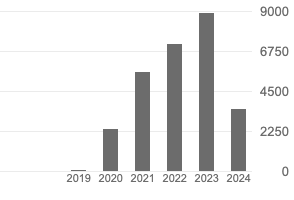
\includegraphics[width=0.5\textwidth]{citation-graph}
\end{minipage}
\end{tabular}



\begin{flushright}\vspace{-5pt}{\footnotesize \it According to Google Scholar on 28th of April, 2024:
  \href{https://scholar.google.com.br/citations?user=5t_sZdMAAAAJ}{\texttt{scholar.google.com.br/citations?user=5t\_sZdMAAAAJ}}}
\end{flushright}



\end{document}

